\section{Linear Functions}
\label{sec:linear}

% Do some regression.
% First differences.
%line 120 - need graph

\subsection{Linear Function Basics}

In Section \ref{ssec:cost}, we had the example of a screen printing shop that charges \$50 to cover the overhead costs of setting the screen to make T-shirts and \$5 per shirt for the shirts themselves. Using descriptive variables, we chose $n$ for the number of T-shirts and $C$ for the cost in dollars as a function of the number of shirts: $C(n)$.

We know that $C(0)$ = 50, since the overhead, or fixed, costs are charged regardless of the number of T-shirts made. Since \$5 is added for each T-shirt ordered, then $C(1) = \$50 + \$5 = \$55$, $C(2) = \$55 + \$5 = \$60$, and so on.

If $n$ T-shirts are ordered, then

$$C(n) = \$50 + \left(\frac{\$5}{\mbox{T-shirt}}\right)(n \mbox{ T-shirts}) = 50 + 5n \mbox{ dollars} \enspace .$$
Notice how the units (or dimensions) make sense in this equation. Each term has units of dollars, after cancelling the unit of ``T-shirt" in the second term.

Notice this equation consisted of two quantities. The first is the fixed \$50 charge which does not change based on the value of the input. When the no T-shirts are ordered, the cost is \$50, giving the point
$(0, 50)$ on the graph of the function. This is the {\bf vertical}\index{Intercept!vertical} or {$y$-intercept}\index{Intercept!$y$}. The second is the \$5 per T-shirt, which is a \textbf{rate of change}\index{Rate of change}. In $C(n)$, this rate of change is multiplied by the input value. It is important here to note that in this equation, the rate of change is {\bf constant}; over any interval, the rate of change is the same.

Looking at $C(n)$ as a table, we can also see the cost changes by \$5 for each additional T-shirt.

\begin{table}[!ht]
\centering
\begin{tabular}{lrrrr}
\toprule
$n$    &  0 &  1 &  2 &  3 \\%\\
\midrule
$C(n)$ & 50 & 55 & 60 & 65 \\%\\
\bottomrule
\end{tabular}
\end{table}

 (Even though we cannot order a fractional number of T-shirts, we still graph $y=C(n)$ on all $n\ge 0$.)

The graph is increasing in a straight line from left to right because for each T-shirt, the cost goes up by \$5; this rate remains consistent.

In this example, you have seen the T-shirt cost modeled in words, an equation, a table, and as a graph. Whenever possible, ensure that you can link these four representations together to continually build your skills. It is important to note that you will not always be able to find all four representations for a problem and so being able to work with all four forms is very important.

The function $C(n)$ is an example of a {\bf linear function}\index{Function!linear}. This name comes from the fact that a graph of a linear function is a line.


\begin{definition}
A \textbf{linear function}\index{Function!linear} is a function whose graph produces a line. Linear functions can always be written in the form
$$f(x) = mx +b \enspace ,$$
where:
    \begin{itemize}
        \item $b$ is the initial or starting value of the function (when the input, $x = 0$), and
        \item $m$ is the constant rate of change of the function.
    \end{itemize}
This form of the line is called the {\bf slope-intercept form}\index{Slope-intercept form}.
\end{definition}

Many people like to write linear functions in the form $y=mx + b$ because it corresponds to the way we tend to speak: ``The output starts at $b$ and increases at a rate of $m$.''

\paragraph*{Slope and Increasing/Decreasing}

The constant rate of change of a linear function, $m$, is also called the \textbf{slope}\index{Slope} of the function. The slope determines if the function is an increasing function or a decreasing function.
\begin{itemize}
  \item $f(x) = mx + b$ is an \textbf{increasing}\index{Increasing} function if $m>0$.
  \item $f(x) = mx + b$ is a \textbf{decreasing}\index{Decreasing} function if $m<0$.
\end{itemize}
If $m=0$, then the rate of change of $f(x) = mx+b$ is zero, and $f(x) = 0\cdot x+b = b$, so its graph is just the horizontal line passing through the point $(0, b)$, neither increasing nor decreasing.

The concepts of slope and rate of change are major component of calculus. It is crucial to understand each facet of these two concpets that we will discuss in this section since these conepts will be generalized from linear functions to a wide array of functions in Chapter \ref{ch:derivatives}.

\begin{example}
Marcus currently owns 200 songs in his iTunes collection. Every month, he adds 15 new songs. Write a formula for the number of songs, $N$, in his iTunes collection as a function of the number of months, $m$. How many songs will he own in a year?

\begin{solution} The initial value for this function is 200, since he currently owns 200 songs, $N(0)=200$ songs. The number of songs increases by 15 songs per month, so the rate of change is 15 songs per month. With this information, we can write the formula:
$$N(m) = 200 \mbox{ songs} + \left(\frac{15\mbox{ songs}}{\mbox{month}}\right)(m \mbox{ months}) = 200 + 15m \mbox{ songs} \enspace .$$

With this formula we can predict how many songs he will have in 1 year (12 months):
$$N(12) = 200 + 15\cdot 12\mbox{ songs}  = 200 + 180 = 380 \mbox{ songs}  \enspace .$$
Marcus will have 380 songs in a year.
\end{solution}\end{example}


\paragraph{Calculating Rate of Change}

Given two values for the input, $x_1$ and $x_2$, and two corresponding values for the output, $y_1$ and $y_2$, or a set of points, $(x_1, y_1)$ and $(x_2, y_2)$, we can find a linear function that contains both points. First we calculate the rate of change, $m$, of the function.

$$\mbox{slope}=\frac{\mbox{rise}}{\mbox{run}}=\frac{\mbox{change in } y}{\mbox{change in } x} \Rightarrow m = \frac{y_2-y_1}{x_2-x_1}$$

It is also customary to write $\Delta v$ for a change (or difference) in the variable $v$. We read this ``delta $v$"\index{Delta ($\Delta$)}. With this notation, we can write
$$m=\frac{\Delta y }{\Delta x} = \frac{y_2-y_1}{x_2-x_1}\enspace .$$

Note in function notation, $y_1 = f(x_1)$ and $y_2 = f(x_2)$, so we could equivalently write
$$m=\frac{f(x_2)-f(x_1)}{x_2-x_1}\enspace .$$

Once we have computed $m$, we can use either of the given points to find $b$ using algebra.
\begin{align*}
y_1 &= mx_1 + b \\
b &= y_1 - mx_1
\end{align*}
\begin{remark} It is a waste of your time to make a special effort to memorize this following formula. This is a concept to understand.
\end{remark}
\begin{example}
The population of a city increased from 23,400 to 27,800 between 2002 and 2006. Find the rate of change of the population during this time span.

\begin{solution} The rate of change will relate the change in population to the change in time. The population increased by $27800-23400 = 4400$ people over the four-year time interval. To find the rate of change, the number of people per year the population changed by:
$$m = \frac{27800-23400 \mbox{ people}}{2006 - 2002 \mbox{ years}} = \frac{4400\mbox{ people}}{4\mbox{ years}} = 1100 \mbox{ people per year} \enspace .$$
\end{solution}\end{example}
Notice that we knew the population was increasing, so we expected $m>0$. This is a quick way to check if the solution is reasonable.

\begin{example}
The pressure, $P$, in pounds per square inch (psi) on a diver depends upon his depth below the water surface, $d$, in feet, following the equation
$$P(d)=14.696+0.434d \enspace .$$
Interpret the components of this function.

\begin{solution} The rate of change, or slope, 0.434 would have units $\frac{\mbox{output}}{\mbox{input}} = \frac{\mbox{pressure}}{\mbox{depth}}=\frac{\mbox{psi}}{\mbox{ft}}$. This tells us the pressure on the diver increases by 0.434 psi for each foot his depth increases.

The initial value, 14.696, will have the same units as the output, so this tells us that at a depth of 0 feet, the pressure on the diver will be 14.696 psi.
\end{solution}\end{example}

We can now find the rate of change given two input-output pairs, and can write an equation for a linear function once we have the rate of change and initial value. If we have two input-output pairs and they do not include the initial value of the function, then we will have to solve for it.

\begin{example}

Write an equation for the linear function graphed below.
%\begin{figure}[!ht]
%\centering
%\includegraphics{images/image048.png}
\begin{center}
\includegraphics[width=0.5\textwidth]{img/chap1/sec1-4/image048.png}
\end{center}
%\caption{}
%\end{figure}

\begin{solution} Looking at the graph, we might notice that it passes through the points $(0, 7)$ and $(4, 4)$. From the first value, we know the initial value of the function is $b = 7$, so in this case we will only need to calculate the rate of change:
$$m = \frac{4-7}{4-0}=\frac{-3}{4} \enspace . $$
This allows us to write the equation:
$$f(x) = 7-\frac{3}{4} x \enspace .$$

\end{solution}\end{example}

\begin{example}
If $f(x)$ is a linear function, $f(3)=-2$, and $f(8) = 1$, find an equation for the function.

\begin{solution} The rate of change (or slope) of the function is $m = \frac{1-(-2)}{8-3} = \frac{3}{5}$. In this case, we do not know the initial value $f(0)$, so we will have to solve for it. Using the rate of change, we know the equation will have the form $f(x)=b+\frac{3}{5}x$. Since we know the value of the function when $x = 3$, we can evaluate the function at 3:
$$f(3)= b + \frac{3}{5}\cdot 3 \enspace.$$
Since we know that $f(3)=-2$, we can substitute on the left side
$$ -2 = b + \frac{3}{5}\cdot 3 \enspace.$$
This leaves us with an equation we can solve for the initial value
$$b = -2 - \frac{9}{5}= -\frac{19}{5} \enspace .$$
Combining this with the value for the rate of change, we can now write a formula for this function:
$$f(x)=-\frac{19}{5} + \frac{3}{5}x\enspace .$$
\end{solution}\end{example}

%As an alternative to the approach used above to find the initial value, b, we can use the point-slope form of a line instead.

%\paragraph{Point-Slope Equation of a Line}
%An equation for the line passing through the point $(x_1, y_1)$ with slope $m$ can be written as
%$$y - y_1 = m(x-x_1)\enspace .$$
%This is called the {\bf point-slope form} of a line. It is a little easier to write if you know a point and the slope, but requires a bit of work to rewrite into slope-intercept form, and requires memorizing another formula.

\begin{example}
Working as an insurance salesperson, Ilya earns a base salary and a commission on each new policy, so his weekly income, $I$, depends on the number of new policies, $n$, he sells during the week. Last week he sold 3 new policies, and earned \$760 for the week. The week before, he sold 5 new policies, and earned \$920. Find an equation for $I(n)$, and interpret the meaning of the components of the equation.

\begin{solution} The given information gives us two input-output pairs: $(3,760)$ and $(5,920)$. We start by finding the rate of change.
$$m = \frac{920-760 \mbox{ dollars}}{5-3\mbox{ policies}}=\frac{160}{2} \mbox{ dollars per policy} = \$80 \mbox{ per policy} \enspace .$$

Keeping track of units, as we did above, can help us interpret this quantity. Income increased by \$160 when the number of policies increased by 2, so the rate of change is \$80 per policy; Ilya earns a commission of \$80 for each policy sold during the week.

We can then solve for the initial value
$I(n) = b + 80n$		then when n = 3, $I(3) = 760$, giving
$760 = b+80\cdot 3 = b + 240$		this allows us to solve for $b$
$b = 760 - 240 = 520$

This form allows us to see the starting value for the function: 520. This is Ilya's income when $n = 0$, which means no new policies are sold. We can interpret this as Ilya's base salary for the week, which does not depend upon the number of policies sold.

Our final interpretation is: Ilya's base salary is \$520 per week and he earns an additional \$80 commission for each policy sold each week.
\end{solution}\end{example}


% \begin{example} Given the table below write a linear equation that represents the table values
%
% We can see from the table that the initial value of rats is 1000 so in the linear format
%
% , $b = 1000$.
%
% Rather than solving for $m$, we can notice from the table that the population goes up by 80 for every 2 weeks that pass. This rate is consistent from week 0, to week 2, 4, and 6. The rate of change is 80 rats per 2 weeks. This can be simplified to 40 rats per week and we can write
%
% as
%
% If you didn't notice this from the table you could still solve for the slope using any two points from the table. For example, using (2, 1080) and (6, 1240),
%
% rats per week
% \end{solution}\end{example}

\subsection{Graphs of Linear Functions}
%\label{section-2.2-graphs-of-linear-functions}

When we are working with a new function, it is useful to know as much as we can about the function: its graph, where the function is zero, and any other special behaviors of the function. We will begin this exploration of linear functions with a look at graphs.

When graphing a linear function, there are two basic ways to graph it.

\begin{enumerate}
\item Plot at least two points and draw a line through the points.
\item Use the initial value (output when $x = 0$) and the rate of change (slope).
\end{enumerate}

\begin{example}
Graph $f(x) = 5 - \frac{2}{3} x$ by plotting points.

\begin{solution} In general, we evaluate the function at two or more inputs to find at
least two points on the graph. Usually it is best to pick input values
that will ``work nicely'' in the equation. In this equation, multiples
of 3 will work nicely due to the in the equation, and of course using
$x = 0$ to get the vertical intercept. Evaluating $f(x)$ at
$x = 0, 3$, and $6$:

$f(0) = 5 - \frac{2}{3} \cdot 0 = 5 $\\
\indent $f(3) = 5 - \frac{2}{3} \cdot 3 = 3 $
\indent $f(6) = 5 - \frac{2}{3} \cdot 6 = 1 $

%%\incluegraphics[width=2.64861in,height=2.26319in]{media/image93.png}

These evaluations tell us that the points $(0,5)$, $(3,3)$, and $(6,1)$ lie on
the graph of the line. Plotting these points and drawing a line through
them gives us the graph.
\end{solution}\end{example}

When using the initial value and rate of change to graph, we need to
consider the graphical interpretation of these values. Remember the
initial value of the function is the output when the input is $0$, so
in the equation $f(x) = b + mx$, the graph includes the point $(0, b)$. On the
graph, this is the vertical intercept -- the point where the graph
crosses the vertical axis.

For the rate of change, it is helpful to recall that we calculated this value as
$$m = \frac{\mbox{change of output}}{\mbox{change of input}}$$
%%\incluegraphics[width=3.00000in,height=2.17986in]{media/image97.png}
From a graph of a line, this tells us that if we divide the vertical
difference, or rise, of the function outputs by the horizontal
difference, or run, of the inputs, we will obtain the rate of change,
also called slope of the line.
$$m = \frac{\mbox{change of output}}{\mbox{change of input}} = \frac{\mbox{rise}}{\mbox{run}}$$


Notice that this ratio is the same regardless of which two points we use.

\paragraph{Graphical Interpretation of a Linear Equation.} Graphically, in the equation, $f(x) = b+mx$,
  \begin{itemize}
    \item $b$ is the \textbf{vertical intercept}\index{Intercept!vertical} of the graph and tells us we can start our graph at $(0, b)$
    \item $m$ is the \textbf{slope of the line}\index{Slope} and tells us how far to rise and run to get to the next point.
  \end{itemize}
Once we have at least two points, we can extend the graph of the line to the left and right.

\begin{example}
Graph $f(x) = 5 - \frac{2}{3} x$ using the vertical intercept and slope.

\begin{solution} The vertical intercept of the function is $(0, 5)$, giving us a point on the graph of the line. The slope is $\dfrac{-2}{3}$. This tells us that for every 3 units the graph ``runs'' in the horizontal, the vertical ``rise'' decreases by 2 units. In graphing, we can use this by first plotting our vertical intercept on the graph, then using the slope to find a second point. From the initial value $(0, 5)$, the slope tells us that if we move to the right 3 units, we will move down 2 units, moving us to the point $(3, 3)$. We can continue this again to find a  third point at $(6, 1)$. Finally, extend the line to the left and right, containing these points.
\begin{figure}[!ht]
\centering
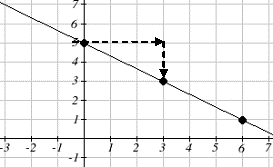
\includegraphics[width=0.5\textwidth]{img/chap1/sec1-4/image049.png}
\caption{}
\end{figure}
\end{solution}\end{example}

Another option for graphing is to use transformations of the identity function $f(x)=x$. In the equation $f(x)=mx$, the $m$ acts as the vertical stretch of the identity function. When $m<0$, there is also a vertical reflection of the graph. Looking at some examples will also help show the effect of slope on the shape of the graph.

\begin{figure}[!ht]
\centering
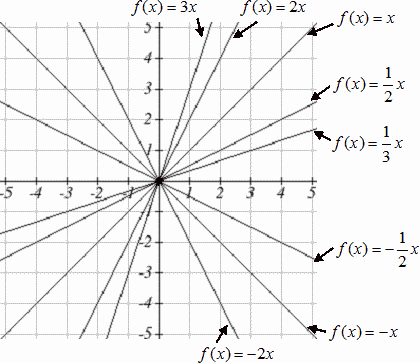
\includegraphics[width=0.5\textwidth]{img/chap1/sec1-4/image050.png}
\caption{$f(x)=mx$ for several values of $m$.}
\end{figure}

In $f(x)=mx+b$, the $b$ acts as the vertical shift, moving the graph up and down without affecting the slope of the line. Here are some examples.

\begin{figure}[!ht]
  \centering
  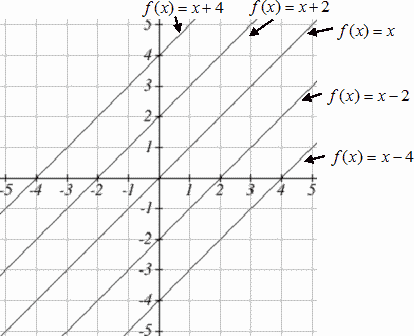
\includegraphics[width=0.5\textwidth]{img/chap1/sec1-4/image051.png}
  \caption{$f(x)=mx$ for several values of $b$.}
\end{figure}

\begin{example}
Match each function with one of the lines in the graph below.
\begin{figure}[!ht]
\centering
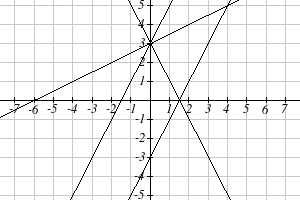
\includegraphics[width=0.5\textwidth]{img/chap1/sec1-4/image052.png}
\caption{}
\end{figure}

\begin{solution} Only one graph has a vertical intercept of $-3$, so we can immediately match that graph with $g(x)$. For the three graphs with a vertical intercept at 3, only one has a negative slope, so we can match that line with $h(x)$. Of the other two, the steeper line would have a larger slope, so we can match that graph with $f(x)$, and the flatter line with $j(x)$.
\begin{figure}[!ht]
\centering
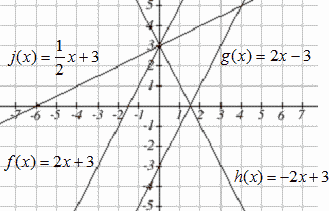
\includegraphics[width=0.5\textwidth]{img/chap1/sec1-4/image095.png}
\caption{}
\end{figure}

\end{solution}\end{example}

In addition to understanding the basic behavior of a linear function (increasing or decreasing, recognizing the slope and vertical intercept), it is often helpful to know the horizontal intercept of the function -- where it crosses the horizontal axis.

\paragraph*{Finding Horizontal Intercepts}

\begin{definition}
  The \textbf{horizontal intercept}\index{Intercept!horizontal} of the function is where the graph crosses the horizontal axis. If a function has a horizontal intercept, you can always find it by solving $f(x) = 0$ for $x$.
\end{definition}

\begin{example}
Find the horizontal intercept of $f(x) = -3 + \frac{1}{2} x$

\begin{solution} Setting the function equal to zero to find what input will put us on the
horizontal axis,
\begin{align*}
  0 &= -3 + \frac{1}{2}x \\
  3 &= \frac{1}{2}x\\
  x &= 6\enspace .
\end{align*}
The graph crosses the horizontal axis at the point $(6,0)$.
\end{solution}\end{example}

\paragraph{Intersections of Lines}

The graphs of two lines will intersect if they are not parallel. They will intersect at the point that satisfies both equations. To find this point when the equations are given as functions, we can solve for an input value so that $f(x)=g(x)$. In other words, we can set the formulas for the lines equal, and solve for the input that satisfies the equation.

Economics tells us that in a free market, the price for an item is related to the quantity that producers will supply and the quantity that consumers will demand. Increases in prices will decrease demand, while supply tends to increase with prices. Sometimes supply and demand are modeled with linear functions.
\begin{example}
  The supply, in thousands of items, for custom phone cases can be modeled by the equation $s(p)=0.5+1.2p$ while the demand can be modeled by $d(p)=8.7−0.7p$, where $p$ is in dollars. Find the equilibrium price and quantity, the intersection of the supply and demand curves.

  \begin{solution} Setting $s(p)=d(p)$, we find
  \begin{align*}
    0.5 + 1.2p &= 8.7−0.7p \\
    1.9p &= 8.2 \\
    p&=\frac{8.2}{1.9} \approx 4.32
  \end{align*}
  We can find the output value of the intersection point by evaluating either function at this input:
  $$ s(4.32) = 0.5+1.2(4.32) \approx 5.68 \enspace .$$
  These lines intersect at the point $(4.32, 5.68)$. Therefore, the equilibrium price is \$4.32 and the equilibrium quantity is 5,680 items. Looking at the graph, this result seems reasonable.
  \begin{figure}[!ht]
  \centering
  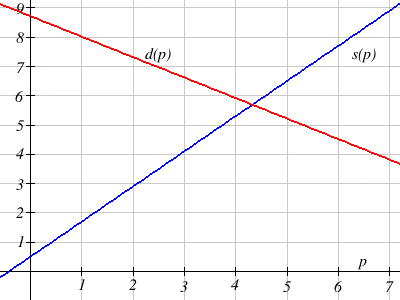
\includegraphics[width=0.5\textwidth]{img/chap1/sec1-4/image053.png}
  \caption{}
  \end{figure}
\end{solution}\end{example}

\subsection{Modeling with Linear Functions}
\label{ssec:modeling-linear}

Here are a number of examples of modeling with linear functions.

\begin{example}

Emily saved up \$3500 for her summer visit to Seattle. She anticipates spending \$400 each week on rent, food, and fun. Find and interpret the horizontal intercept and determine a reasonable domain and range for this function.

\begin{solution} In the problem, there are two changing quantities: time and money. The amount of money she has remaining while on vacation depends on how long she stays. We can define our variables, including units.
  \begin{itemize}
    \item[] {\bf Output:} $M$, money remaining, in dollars
    \item[] {\bf Input:} $t$, time, in weeks
  \end{itemize}
Reading the problem, we identify two important values. The first, \$3500, is the initial value for $M$. The other value appears to be a rate of change -- the units of dollars per week match the units of our output variable divided by our input variable. She is spending money each week, so you should recognize that the amount of money remaining is
decreasing each week and the slope is negative.

To answer the first question, looking for the horizontal intercept, it would be helpful to have an equation modeling this scenario. Using the intercept and slope provided in the problem, we can write the equation: $M(t) = 3500-400t$.

To find the horizontal intercept, we set the output to zero, and solve for the input, $t$:
\begin{align*}
  0 &= 3500  - 400 t \\
  400t &= 3500 \\
  t &= \frac{3500}{400} = 8.75
\end{align*}
The horizontal intercept is 8.75 weeks. Since this represents the input value where the output will be $0$, interpreting this, we could say: ``Emily will have no money left after 8.75 weeks."

When modeling any real life scenario with functions, there is typically a limited domain over which that model will be valid -- almost no trend continues indefinitely. In this case, it certainly doesn't make sense to talk about input values less than $0$. It is also likely that this model is not valid after the horizontal intercept (unless Emily's going to start using a credit card and go into debt).

The domain represents the set of input values and so the reasonable domain for this function is $0\le t\le 8.75$.

However, in a real world scenario, the rental might be weekly or nightly. She may not be able to stay a partial week and so all options should be considered. Emily could stay in Seattle for 0 to 8 full weeks (and a couple of days), but would have to go into debt to stay 9 full weeks, so restricted to whole weeks, a reasonable domain without going
in to debt would be $0\le t\le 8$, or $0\le t\le 9$ if she went into debt to finish out the last week.

The range represents the set of output values and she starts with \$3500 and ends with \$0 after 8.75 weeks so the corresponding range is $0\le M(t)\le 3500$. If we limit the rental to whole weeks, however, the range would change. If she left after 8 weeks because she didn't have enough to stay for a full 9 weeks, she would have $M(8) = 3500-400\cdot 8 = \$300$ left after 8 weeks, giving a range of $300\le M(t)\le 3500$. If she wanted to stay the full 9 weeks she would be \$100 in debt giving a range of $-100\le M(t)\le 3500$.
\end{solution}\end{example}

Most importantly remember that domain and range are tied together, and what ever you decide is most appropriate for the domain (the independent variable) will dictate the requirements for the range (the dependent variable).

\begin{example}
Jamal is choosing between two moving companies. The first, U-Haul, charges an up-front fee of \$20, then 59 cents per mile. The second, Budget, charges an up-front fee of \$16, then 63 cents per mile.\footnote{Rates retrieved Aug 2, 2010 from \url{http://www.budgettruck.com} and \url{http://www.uhaul.com/}.} When will U-Haul be the better choice
for Jamal?

\begin{solution} The two important quantities in this problem are the cost, and the number of miles that are driven. Since we have two companies to consider, we will define two functions:
  \begin{itemize}
    \item[] {\bf Input:} $m$, miles driven
    \item[] {\bf Outputs:}
      \begin{itemize}
        \item[] $Y(m)$: cost, in dollars, for renting from U-Haul
        \item[] $B(m)$: cost, in dollars, for renting from Budget
      \end{itemize}
    \end{itemize}
Reading the problem carefully, it appears that we were given an initial cost and a rate of change for each company. Since our outputs are measured in dollars but the costs per mile given in the problem are in cents, we will need to convert these quantities to match our desired units: \$0.59 per mile for U-Haul, and \$0.63 per mile for Budget.

%\incluegraphics[width=2.75417in,height=2.70903in]{media/image245.png}
Looking to what we're trying to find, we want to know when U-Haul will be the better choice. Since all we have to make that decision from is the costs, we are looking for when U-Haul will cost less, or when $Y(m) < B(m)$. The solution pathway will lead us to find the equations for the two functions, find the intersection, then look to see where $Y(m)$ is smaller. Using the rates of change and initial charges, we can write the equations:
\begin{align*}
  Y(m) &= 20 + 0.59 m\\
  B(m) &= 16 + 0.63 m
\end{align*}
These graphs are sketched to the right, with $Y(m)$ drawn dashed.

[INSERT GRAPH]
%\incluegraphics[width=2.75417in,height=2.70903in]{media/image245.png}
To find the intersection, we set the equations equal to each other and solve for $m$.
\begin{align*}
  Y(m) &= B(m) \\
  20 + 0.59 m &= 16 + 0.63 m\\
  4 &= 0.04 m\\
  m &= \frac{4}{0.04} = 100
\end{align*}

This tells us that the cost from the two companies will be the same if you drive 100 miles. Either by looking at the graph, or noting that $Y(m)$ is growing at a slower rate, we can conclude that U-Haul would be the cheaper option if you drive more than 100 miles.
\end{solution}\end{example}
\begin{example}
A town's population has been growing linearly. In 2004 the population was 6,200. By 2009 the population had grown to 8,100. If this trend continues,
  \begin{enumerate}[label={\alph*)}]
    \item Predict the population in 2013.
    \item When will the population reach 15,000?
  \end{enumerate}

\begin{solution} The two changing quantities are the population and time. While we could use the actual year value as the input quantity, doing so tends to lead to very ugly equations, since the vertical intercept would correspond to
the year 0, more than 2000 years ago!

To make things a little nicer, and to make our lives easier too, we will define our input as years since 2004.
  \begin{itemize}
      \item[] {\bf Input:} $t$, years since 2004
      \item[] {\bf Output:} $P(t)$, the town's population
    \end{itemize}
The problem gives us two input-output pairs. Converting them to match our defined variables, the year 2004 would correspond to $t = 0$, giving the point $(0, 6200)$. Notice that through our clever choice of variable definition, we have ``given'' ourselves the vertical intercept of the function. The year 2009 would correspond to $t = 5$, giving us
the point $(5, 8100)$.

\begin{enumerate}[label={\alph*)}]
  \item To predict the population in 2013 ($t = 9$), we would need an equation for the population. Likewise, to find when the population would reach 15000, we would need to solve for the input that would provide an output of 15000. Either way, we need an equation. To find it, we start by calculating the rate of change:
$$m = \frac{8100-6200}{5-0} = \frac{1900}{5} = 380 \mbox{ people per year .}$$

Since we already know the vertical intercept of the line, we can immediately write the equation:
$$P(t) = 6200 +380t \enspace .$$
To predict the population in 2013, we evaluate our function at $t = 9$:
$$P(9) = 6200 +380 \cdot 9 = 9620 \enspace .$$
If the trend continues, our model predicts a population of 9,620 in 2013.

  \item To find when the population will reach 15,000, we can set $P(t) = 15000$ and solve for $t$.
\begin{align*}
  P(t) &= 15000 \\
  6200 +380t &= 15000 \\
  380 t &= 8800 \\
  t &= \frac{8800}{380} \approx 23.158
\end{align*}
Our model predicts the population will reach 15,000 in a little more than 23 years after 2004, or somewhere around the year 2027.
\end{enumerate}
\end{solution}\end{example}

\subsection{Fitting Linear Models to Data}
\label{ssec:linear-models-data}

In the real world, things rarely follow trends perfectly. When we expect the trend to behave linearly, or when inspection suggests the trend is behaving linearly, it is often desirable to find an equation to approximate the data. Finding an equation to approximate the data helps us understand the behavior of the data and allows us to use a linear model to make predictions about the data, inside and outside of the data range.

\begin{example}
The table below shows the number of cricket chirps in 15 seconds, and the air temperature, in degrees Fahrenheit\footnote{Selected data from \url{http://classic.globe.gov/fsl/scientistsblog/2007/10/}. Retrieved Aug 3, 2010}. Plot this data, and determine whether the data appears to be linearly related.
\begin{table}[!ht]
  \centering
  \begin{tabular}{llllllllll}
    \toprule
    Chirps & 44 & 35 & 20.4 & 33 & 31 & 35 & 18.5 & 37 & 26 \\
    \midrule
    Temp. ($^{\circ}$F) & 80.5 & 70.5 & 57 & 66 & 68 & 72 & 52 & 73.5 & 53\\
    \bottomrule
  \end{tabular}
  \caption{Cricket Chirps in 15 Seconds Versus Temperature.}
\end{table}

\begin{solution} Plotting this data, it appears there may be a trend, and that the trend appears roughly linear, though certainly not perfectly so. We will plot this data in a spreadsheet. First, we put the data in a spreadsheet.

  \begin{table}[!ht]
    \centering
    \textsf{
    \begin{tabular}{|a*{10}{|c}|}
      \hline
      \rowcolor{shGray} & A & B & C & D & E & F & G & H & I & J\\
      \hline
        1 & \textbf{Chirps} & 44 & 35 & 20.4 & 33 & 31 & 35 & 18.5 & 37 & 26 \\
      \hline
        2 & \textbf{Temp. ($^{\circ}$F)} & 80.5 & 70.5 & 57 & 66 & 68 & 72 & 52 & 73.5 & 53\\
      \hline
    \end{tabular}}
    \caption{}
    \label{sh:crickets}
  \end{table}
  First we make a scatter plot. See Section \ref{ssec:plot-data} for the details on how we create a scatterplot in {\em LibreOffice Calc}.
  \begin{remark}
    The default scatter plot is on the left and a revised plot is on the right. Notice that the default plot includes a lot of unnecessary ``white space," with a range of $0\degF$ to $90\degF$. A more reasonable range is $50\degF$ to $85\degF$. Within {\em Calc}, clicking on the $y$-axis will allow us to adjust the chart to make it more presentable. We can likewise trim the domain slightly.
  \end{remark}

    \begin{center}
    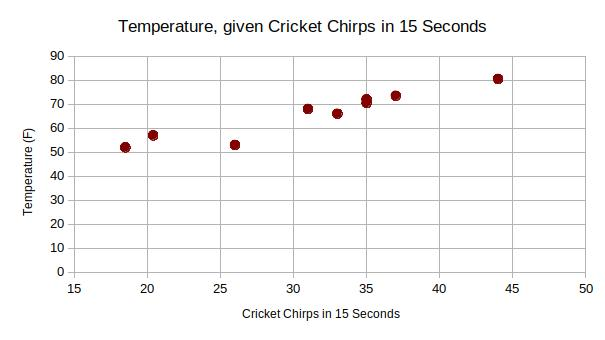
\includegraphics[width = 0.49\textwidth]{img/chap1/sec1-4/1-4-crickets-plot1.jpg}~
    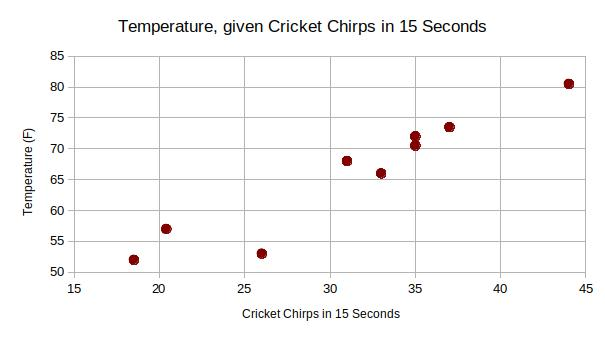
\includegraphics[width = 0.49\textwidth]{img/chap1/sec1-4/1-4-crickets-plot2.jpg}
    \end{center}

\end{solution}\end{example}

The simplest way to find an equation to approximate this data is to try to ``eyeball'' a line that seems to fit the data pretty well, then find an equation for that line based on the slope and intercept.

You can see from the trend in the data that the number of chirps increases as the temperature increases. As you consider a function for this data you should know that you are looking at an increasing function or a function with a positive slope.

{\bf Questions to Consider:}
  \begin{itemize}
    \item What descriptive variables would you choose to represent temperature and chirps?
    \item Which variable is the independent variable and which is the dependent variable?
    \item Based on this data and the graph, what is a reasonable domain and range?
  \end{itemize}

\begin{example}
\label{ex:1-4-crickets}
Using the table of values from the previous example, find a linear function that fits the data by ``eyeballing'' a line that seems to fit.

\begin{solution} On a graph, we could try sketching in a line. The figure below has a rough line that approximates the trend of the data.
  \begin{center}
  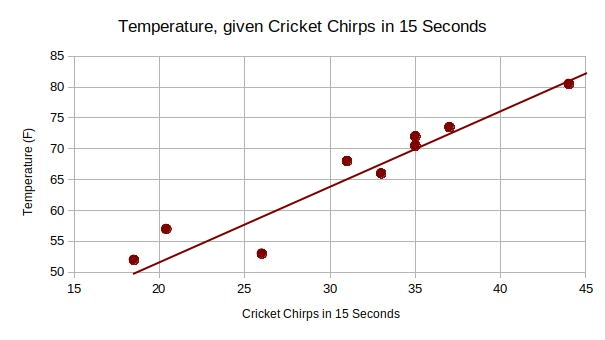
\includegraphics[width = 0.6\textwidth]{img/chap1/sec1-4/1-4-crickets-plot-handline.jpg}
  \end{center}

To find an equation of the line, we pick two points on the line. The best places to pick points are he intersection of grid lines, such as $(35, 70)$. Others would be points near extreme points of the line on a grid line, such as $(20, 52)$ and $(45, 82)$; 52 and 82 are estimates. Based on these latter two points, the line has a slope of $m = \dfrac{82-52}{45-20} = \dfrac{30}{25} = 1.2$. Now we find the vertical intercept at 30. Since the line has an equation of the form $y = 1.2 x+b$ and one point has $x=35$ and $y=70$, we have
\begin{align*}
  70 &= 1.2\cdot 35 + b\\
  &= 42 + b\\
  b &= 70-42 = 28 \enspace .
\end{align*}
This gives us the model
$$T(c) = 28 + 1.2 c \enspace, $$
where $c$ is the number of chirps in 15 seconds, and $T(c)$ is the temperature in degrees Fahrenheit.
\end{solution}\end{example}

This linear equation can then be used to approximate the solution to various questions we might ask about the trend. While the data does not perfectly fall on the linear equation, the equation is our best guess as to how the relationship will behave outside of the values we have data for. Recall the notions of interpolation and extrapolation.

\begin{example}
  \begin{itemize}
    \item[a)] Would predicting the temperature when crickets are chirping 30 times in 15 seconds be interpolation or extrapolation? Make the prediction, and discuss if it is reasonable.
    \item[b)] Would predicting the number of chirps crickets will make at 40 degrees be interpolation or extrapolation? Make the prediction, and discuss if it is reasonable.
  \end{itemize}

  \begin{solution}
    \begin{itemize}
        \item[a)] With our cricket data, the number of chirps in the data provided varied from 18.5 to 44. A prediction at 30 chirps per 15 seconds is inside the domain of our data, so this would be a case of interpolation. Using our model:
        $$T(28) = 28 + 1.2\cdot 30 = 64^{\circ}\mbox{F .}$$
        Based on the data we have, this value seems reasonable.

        \item[b)] The temperature values varied from $52^{\circ}\mbox{F}$ to $80.5^{\circ}\mbox{F}$. Predicting the number of chirps at 40 degrees is extrapolation since 40 is outside the range of our data. Using our model:
        \begin{align*}
          40 &= 28 + 1.2c\\
          12 &= 1.2 c\\
          c &= \frac{12}{1.2} \approx 10
        \end{align*}
        Our model predicts the crickets would chirp 10 times in 15 seconds. While this might be possible, we have no reason to believe our model is valid outside the domain and range. In fact, crickets generally stop chirping altogether below around $50^{\circ}\mbox{F}$. Therefore, our prediction is likely unreasonable.
      \end{itemize}
\end{solution}\end{example}


%Try it Now
%
%1. What temperature would you predict if you counted 20 chirps in 15 seconds?

\subsection{Fitting Lines with a Spreadsheet.}
In this section, we will use {\em LibreOffice Calc} to compute the {\bf line of best fit} or {\bf regression line}\index{Line!best fit}\index{Line!regression}\index{Regression!line} for various data sets.

\begin{example}
Find the least-squares regression line using the cricket chirp data from Table \ref{sh:crickets}.

\begin{solution} Double-click on the chart made from the data in Table \ref{sh:crickets}.
  \begin{itemize}
    \item Click on a data point so that the points turn green.
    \item Select the menu item {\tt Trend Line...}. This will bring up a regression curve wizard.
    \item Click on the {\tt Type} tab.
    \item Make the selections given in Figure \ref{fig:lin-reg-menu}.
  \end{itemize}
  \begin{figure}[!ht]
        \centering
        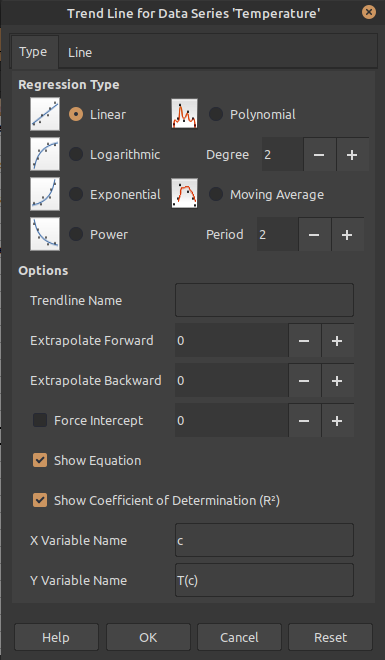
\includegraphics[width=0.4\textwidth]{img/chap1/sec1-4/lin-reg-crickets-menu.png}
        \caption{}
        \label{fig:lin-reg-menu}
  \end{figure}
  The new scatter plot in Figure \ref{fig:lin-reg-crickets} now has the linear regression line. By default, the regression line has far too much precision than we need for this context. Two decimal place of precision is enough. We can make that change by clicking on the equation for the line of best fit and going to the {\tt Numbers} tab.
  \begin{figure}[!ht]
    \centering
      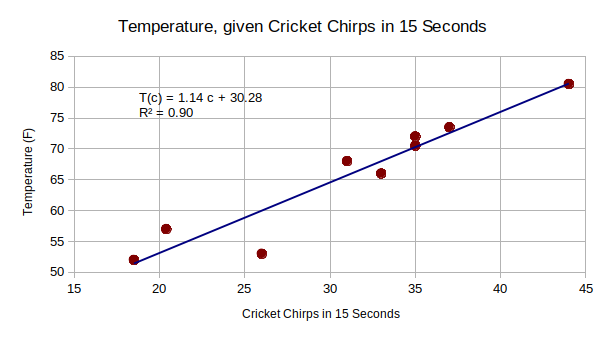
\includegraphics[width=0.6\textwidth]{img/chap1/sec1-4/lin-reg-crickets.png}
      \caption{}
      \label{fig:lin-reg-crickets}
  \end{figure}
  Therefore, the best-fit line is
$$T(c) = 1.14 c + 30.28 \mbox{ degrees Fahrenheit.}$$
This line is very similar to the equation we ``eyeballed,'' but it fits the data better. Notice also that using this equation would change our prediction for the temperature when hearing 30 chirps in 15 seconds from 66 degrees to:
$$T(30) = 1.14\cdot 30 + 30.28 = 64.48\degF \enspace .$$
\end{solution}\end{example}

Notice that the plot also includes another number: $R^2 = 0.90$. Most calculators and computer software will also provide you with this number, called the {\bf coefficient of determination}\index{Coefficient of determination}, or the related \textbf{correlation coefficient}\index{Correlation coefficient}. These numbers measure how well a function models a set of data.

\begin{definition}[Correlation Coefficient]
  The \textbf{correlation coefficient} is a value, $-1 \le r \le 1$ that measures the strength of the relationship between two variables, $x$ and $y$. $|r|$ measures the proportion of the output variable, $y$, can be explained by the input variable, $x$.
  \begin{itemize}
  \item $r  >  0$ suggests a positive (increasing) relationship between $x$ and $y$.
  \item $r  <  0$ suggests a negative (decreasing) relationship between $x$ and $y$.
  \item The closer $r$ is to 0, the more scattered or {\bf noncorrelated} the data.
  \item The closer $r$ is to 1 or $-1$, the stronger the relationship the data is.
\end{itemize}
  The {\bf coefficient of determination} is the value $0\le r^2 \le 1$, which measures the proportion of the variable $y$ that is determined, or predicted, by $x$.
\end{definition}

We should only compute the correlation coefficient for data that follows a linear pattern; if the data exhibits a non-linear pattern, the correlation coefficient is meaningless. To get a sense for the relationship between the value of $r$ and the graph of the data, here are some large data sets with their correlation coefficients:
[Provide graph]
%\incluegraphics[width=5.82292in,height=2.44792in]{media/image301.png}\footnote{\url{http://en.wikipedia.org/wiki/File:Correlation_examples.png}}


\begin{example}
  The coefficient of determination of the cricket chirp data is $r^2 = 0.90$. Since the linear regression line has a positive slope, the correlation coefficient is $r = \sqrt{0.9} = 0.95$. This is a very strong relationship between a cricket's chirp rate and the temperature. \hfill $\blacksquare$
\end{example}

We can compute the correlation coefficient directly in {\em Calc}.
\begin{example}
  Compute the correlation coefficient of the following data, repeated from Table \ref{sh:crickets}.
  \begin{table}[!ht]
    \centering
    \textsf{
    \begin{tabular}{|a*{10}{|c}|}
      \hline
      \rowcolor{shGray} & A & B & C & D & E & F & G & H & I & J\\
      \hline
        1 & \textbf{Chirps} & 44 & 35 & 20.4 & 33 & 31 & 35 & 18.5 & 37 & 26 \\
      \hline
        2 & \textbf{Temp. ($^{\circ}$F)} & 80.5 & 70.5 & 57 & 66 & 68 & 72 & 52 & 73.5 & 53\\
      \hline
    \end{tabular}}
  \end{table}
  \begin{solution}
    In a new box, type the following command and hit {\tt Enter}.
    \begin{center}
      \framebox[1.1\width]{\tt =CORREL(B1:J1, B2:J2)}
    \end{center}
    We find $r = 0.9509$.
  \end{solution}\end{example}

\begin{example}
Gasoline consumption in the US has been increasing steadily. Consumption data from 1994 to 2004 is shown below.\footnote{http://www.bts.gov/publications/national\_transportation\_statistics/2005/html/table\_04\_10.html}
Determine if the trend is linear, and if so, find a model for the data. Use the model to predict the consumption in 2008.

\begin{table}[!ht]
  \centering
  \resizebox{\textwidth}{!}{%
  \begin{tabular}{lccccccccccc}
    \toprule
    {\bf Year} & '94 & '95 & '96 & '97 & '98 & '99 & '00 & '01 & '02 & '03 & '04 \\
    \midrule
    {\bf Gasoline consumption (billion gallons)} & 113 & 116 & 118 & 119 & 123 & 125 & 128 & 126 & 131 & 133 & 136\\
    \bottomrule
  \end{tabular}}
  \caption{Gasoline consumption in the United States from 1994 to 2004.}
\end{table}

\begin{solution} To make things simpler, a new input variable is introduced, $t$, representing years since 1994. We make the following spreadsheet.

  \begin{table}[!ht]
    \centering
    \textsf{
    \begin{tabular}{|a*{12}{|c}|}
      \hline
      \rowcolor{shGray} & A & B & C & D & E & F & G & H & I & J & K & L\\
      \hline
        1 & \textbf{Year} & 0 & 1 & 2 & 3 & 4 & 5 & 6 & 7 & 8 & 9 & 10 \\
      \hline
        2 & \textbf{Gas Consumption} & 113 & 116 & 118 & 119 & 123 & 125 & 128 & 126 & 131 & 133 & 136\\
      \hline
    \end{tabular}}
  \end{table}

The following is a scatterplot of the data.
  \begin{center}
    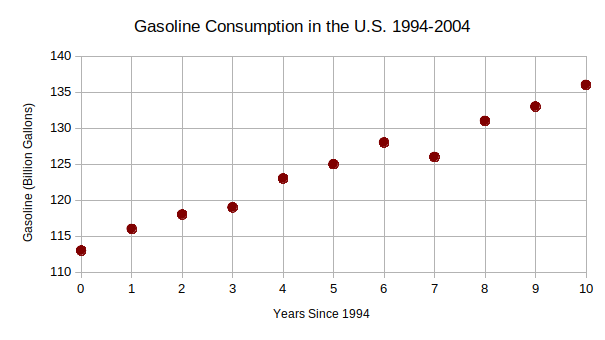
\includegraphics[width=0.6\textwidth]{img/chap1/sec1-4/gas.png}
  \end{center}
The data appears linear. Let's compute the correlation coefficient.
  \begin{center}
    \framebox[1.1\width]{\tt =CORREL(B1:L1, B2:L2)}
  \end{center}
We have $r = 0.9883$, suggesting a very strong increasing linear trend.

Let $t$ be the number of years since 1994 and $C(t)$ be the volume of gasoline consumed in the United States, in billions of gallons. Then the least-squares regression equation is:
$$C(t) = 113.41 + 2.19t \enspace .$$
Here is the scatter plot with the best fit line.
\begin{center}
  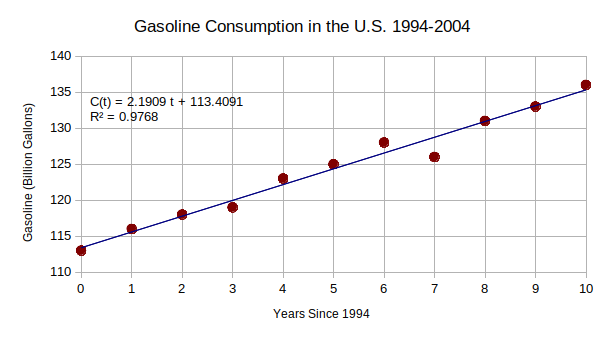
\includegraphics[width=0.6\textwidth]{img/chap1/sec1-4/gas-line.png}
\end{center}

Using this to predict gasoline consumption in 2008 ($t = 14$), we have
$$C(14) = 113.41 + 2.19\cdot 14 = 144.07 \mbox{ billion gallons.}$$


\end{solution}\end{example}

% Try it Now
%
% 2. Use the model created by technology in example 6 to predict the gas
% consumption in 2011. Is this an interpolation or an extrapolation?
%
% Important Topics of this Section
%
% Fitting linear models to data by hand
%
% Fitting linear models to data using technology
%
% Interpolation
%
% Extrapolation
%
% Correlation coefficient
%
% Flashback Answers
%
% 1. a. T = Temperature, C = Chirps (answers may vary)
%
% b. Independent (Chirps) , Dependent (Temperature)
%
% c. Reasonable Domain (18.5, 44) , Reasonable Range (52, 80.5) (answers
% may vary)
%
% d. NO, it is not one-to-one, there are two different output values for
% 35 chirps.
%
% Try it Now Answers
%
% 1. 54 degrees Fahrenheit
%
% 2. 150.871 billion gallons; extrapolation

\subsection{Exercises}
\label{1-4-exercises}

% Try it Now
%
% 1. If you earn \$30,000 per year and you spend \$29,000 per year write
% an equation for the amount of money you save after $y$ years, if
% you start with nothing.\\
% $``The most important thing, spend less than you earn!}\footnote{\url{http://www.thesimpledollar.com/2009/06/19/rule-1-spend-less-than-you-earn/}}$''}


\begin{enumerate}

\item A town's population has been growing linearly. In 2003, the population was 45,000, and the population has been growing by 1700 people each year. Write an equation,for the population $t$ years after 2003.

\item A town's population has been growing linearly. In 2005, the population was 69,000, and the population has been growing by 2500 people each year. Write an equation,for the population $t$ years after 2005.

\item Sonya is currently 10 miles from home, and is walking away from home at 3 miles per hour. Write an equation for her distance from home $t$ hours from now.

\item A boat is 100 miles away from the marina, sailing directly towards it at 10 miles per hour. Write an equation for the distance of the boat from the marina after $t$ hours.

\item Timmy goes to the fair with \$40. Each ride costs \$2. How much money will he have left after riding $n$ rides?

\item At noon, a barista notices she has \$20 in her tip jar. If she makes an average of \$0.50 from each customer, how much will she have in her tip jar if she serves $n$ more customers during her shift?


% Determine if each function is increasing or decreasing
%
% \item. \item.
%
% 9. 10.
%
% 11. 12.
%
% 13. 14.
%
% 15. 16.
%
% Find the slope of the line that passes through the two given points [make into an application with units.]
%
% \item. $(2, 4)$ and $(4, 10)$
%
% \item $(1, 5)$ and $(4, 11)$
%
% 19. (-1,4) and (5, 2) 20. (-2, 8) and (4, 6)
%
% 21. (6,11) and (-4,3) 22. (9,10) and (-6,-12)
%
% Find the slope of the lines~graphed
%
% 23.
% %%\incluegraphics[width=1.94444in,height=1.91516in]{media/image68.png}
% 24.
% %%\incluegraphics[width=1.93264in,height=1.94382in]{media/image69.png}
%
%
% \item Sonya is walking home from a friend's house. After 2 minutes she is 1.4 miles from home. Twelve minutes after leaving, she is 0.9 miles from home. How fast is she walking?
%
% \item A monthly gym membership with two personal training sessions costs \$125, while gym membership with 5 personal training sessions costs \$260. What is the rate for personal training sessions?
%
% \item A city's population in the year 1960 was 287,500. In 1989 the population was 275,900. Compute the slope of the population growth (or decline) and make a statement about the population rate of change in people per year.
%
% \item A city's population in the year 1958 was 2,113,000. In 1991 the population was 2,099,800. Compute the slope of the population growth (or decline) and make a statement about the population rate of change in people per year.
%
% \item A phone company charges for service according to the formula: , where $n$ is the number of minutes talked, and is the monthly charge, in dollars.
%     \begin{enumerate}
%         \item Find the rate of change and initial value.
%         \item What does your answer in part (a) mean in the context of the problem?
%     \end{enumerate}
%
% \item  A phone company charges for service according to the formula: , where $n$ is the number of minutes talked, and is the monthly charge, in dollars.
%     \begin{enumerate}
%         \item Find the rate of change and initial value.
%         \item What does your answer in part (a) mean in the context of the problem?
%     \end{enumerate}
%
% \item Terry is skiing down a steep hill. Terry's elevation, , in feet after $t$ seconds is given by . Write a complete sentence describing Terry's starting elevation and how it is changing over time.
%
% \item Maria is climbing a mountain. Maria's elevation, , in feet after $t$ minutes is given by . Write a complete sentence describing Maria's starting elevation and how it is changing over time.\\
%
% Given each set of information, find a linear equation satisfying the
% conditions, if possible
%
% 33. , and 34. , and
%
% 35. Passes through (2, 4) and (4, 10) 36. Passes through (1, 5) and (4,
% 11)
%
% 37. Passes through (-1,4) and (5, 2) 38. Passes through (-2, 8) and (4,
% 6)
%
% 39. $x$ intercept at (-2, 0) and $y$ intercept at (0, -3)
%
% 40. $x$ intercept at $(-5, 0)$ and $y$ intercept at (0, 4)
%
% Find an equation for the function graphed
%
% 41.
% %\incluegraphics[width=1.97983in,height=1.95000in]{media/image68.png}
% 42.
% %\incluegraphics[width=1.93878in,height=1.95000in]{media/image69.png}
%
% 43.
% %\incluegraphics[width=1.91233in,height=1.95000in]{media/image82.png}
% 44.
% %\incluegraphics[width=1.92549in,height=1.95000in]{media/image83.png}
%
%
% \def\labelenumi{\arabic{enumi}.}
% \setcounter{enumi}{44}
% \item
%   A clothing business finds there is a linear relationship between the
%   number of shirts, $n$, it can sell and the price, $p$, it
%   can charge per shirt. In particular, historical data shows that shirts
%   can be sold at a price of , while shirts can be sold at a price of .
%   Find a linear equation in the form that gives the price $p$ they
%   can charge for $n$ shirts.
% \item
%   A farmer finds there is a linear relationship between the number of
%   bean stalks, $n$, she plants and the yield, $y$, each plant
%   produces. When she plants 30 stalks, each plant yields 30 oz of beans.
%   When she plants 34 stalks, each plant produces 28 oz of beans. Find a
%   linear relationships in the form that gives the yield when $n$
%   stalks are planted.
%
% \item
%   Which of the following tables could represent a linear function? For
%   each that could be linear, find a linear equation models the data.
%
% \begin{table}[!ht]
% \centering
% \begin{tabular}{cccc}
% \toprule
% \begin{minipage}[t]{0.24\columnwidth}\raggedright\strut
% \begin{table}[!ht]
% \centering
% \begin{tabular}{rr}
% \toprule
% $x$ & $g(x)$\\
% \midrule
% 0 & 5\\
% 5 & -10\\
% 10 & -25\\
% 15 & -40\\
% \bottomrule
% \end{tabular}
% \end{table}\strut
% \end{minipage} & \begin{minipage}[t]{0.24\columnwidth}\raggedright\strut
% \begin{table}[!ht]
% \centering
% \begin{tabular}{rr}
% \toprule
% $x$ & $h(x)$\\
% \midrule
% 0 & 5\\
% 5 & 30\\
% 10 & 105\\
% 15 & 230\\
% \bottomrule
% \end{tabular}
% \end{table}\strut
% \end{minipage} & \begin{minipage}[t]{0.24\columnwidth}\raggedright\strut
% \begin{table}[!ht]
% \centering
% \begin{tabular}{rr}
% \toprule
% $x$ & $f(x)$\\
% \midrule
% 0 & $-5$\\
% 5 & 20\\
% 10 & 45\\
% 15 & 70\\
% \bottomrule
% \end{tabular}
% \end{table}\strut
% \end{minipage} & \begin{minipage}[t]{0.24\columnwidth}\raggedright\strut
% \begin{table}[!ht]
% \centering
% \begin{tabular}{rr}
% \toprule
% $x$ & $k(x)$\\
% \midrule
% 5 & 13\\
% 10 & 28\\
% 20 & 58\\
% 25 & 73\\
% \bottomrule
% \end{tabular}
% \end{table}\strut
% \end{minipage}\\
% \bottomrule
% \end{tabular}
% \end{table}
%
% \item
%   Which of the following tables could represent a linear function? For
%   each that could be linear, find a linear equation models the data.
%
% \begin{table}[]
% \begin{tabular}{cccc}
% \toprule
% \begin{minipage}[t]{0.24\columnwidth}\raggedright\strut
% \begin{table}[!ht]
% \centering
% \begin{tabular}{rr}
% \toprule
% $x$ & $g(x)$\\
% \midrule
% 0 & 6\\
% 2 & $-19$\\
% 4 & $-44$\\
% 6 & $-69$\\
% \bottomrule
% \end{tabular}
% \end{table}\strut
% \end{minipage} & \begin{minipage}[t]{0.24\columnwidth}\raggedright\strut
% \begin{table}[!ht]
% \centering
% \begin{tabular}{rr}
% \toprule
% $x$ & $h(x)$\\
% \midrule
% 2 & 13\\
% 4 & 23\\
% 8 & 43\\
% 10 & 53\\
% \bottomrule
% \end{tabular}
% \end{table}\strut
% \end{minipage} & \begin{minipage}[t]{0.24\columnwidth}\raggedright\strut
% \begin{table}[!ht]
% \centering
% \begin{tabular}{rr}
% \toprule
% $x$ & $f(x)$\\
% \midrule
% 2 & $-4$\\
% 4 & 16\\
% 6 & 36\\
% 8 & 56\\
% \bottomrule
% \end{tabular}
% \end{table}\strut
% \end{minipage} & \begin{minipage}[t]{0.24\columnwidth}\raggedright\strut
% \begin{table}[!ht]
% \centering
% \begin{tabular}{rr}
% \toprule
% $x$ & $k(x)$\\
% \midrule
% 0 & 6\\
% 2 & 31\\
% 6 & 106\\
% 8 & 231\\
% \bottomrule
% \end{tabular}
% \end{table}\strut
% \end{minipage}\\
% \bottomrule
% \end{tabular}
% \end{table}
%
% \item
%   While speaking on the phone to a friend in Oslo, Norway, you learned
%   that the current temperature there was $-23^{\circ}$C. After the phone conversation, you wanted to
%   convert this temperature to Fahrenheit, $^{\circ}$F, but you could not find a reference with the correct formulas. You then remembered that the relationship between $^{\circ}$F and
%   $^{\circ}$C is linear. {[}UW{]}
%
% \item
%   Using this and the knowledge that 32$^{\circ}$F = 0
%   $^{\circ}$C and 212 $^{\circ}$F = 100
%   $^{\circ}$C, find an equation that computes Celsius
%   temperature in terms of Fahrenheit; i.e. an equation of the form C =
%   ``an expression involving only the variable F.''
% \item
%   Likewise, find an equation that computes Fahrenheit temperature in
%   terms of Celsius temperature; i.e. an equation of the form F = ``an
%   expression involving only the variable C.''
% \item
%   How cold was it in Oslo in $^{\circ}$F?
%
%
% Match each linear equation with its graph
%
% %\incluegraphics[width=2.16250in,height=2.21319in]{media/image160.png}
%
%
%
% Sketch a line with the given features
%
% \item
%   An $x$-intercept of (-4, 0) and $y$-intercept of (0, -2)
% \item
%   An $x$-intercept of (-2, 0) and $y$-intercept of (0, 4)
% \item
%   A vertical intercept of (0, 7) and slope
% \item
%   A vertical intercept of (0, 3) and slope
% \item
%   Passing through the points (-6,-2) and (6,-6)
% \item
%   Passing through the points (-3,-4) and (3,0)
%
%
% Sketch the graph of each equation
%
% 13. 14.
%
% 15. 16.
%
% 17. 18.
%
% 19. 20.
%
% 21. 22.
%
% ~
%
% \def\labelenumi{\arabic{enumi}.}
% \setcounter{enumi}{22}
% \item
%   If is the transformation of after a vertical compression by , a shift
%   left by 2, and a shift down by 4
%
%   \begin{enumerate}
%   \def\labelenumii{\alph{enumii}.}
%   \item
%     Write an equation for
%   \item
%     What is the slope of this line?
%   \item
%     Find the vertical intercept of this line.
%   \end{enumerate}
% \item
%   ~If is the transformation of after a vertical compression by , a shift
%   right by 1, and a shift up by 3
%
%   \begin{enumerate}
%   \def\labelenumii{\alph{enumii}.}
%   \item
%     Write an equation for
%   \item
%     What is the slope of this line?
%   \item
%     Find the vertical intercept of this line.
%   \end{enumerate}
%
% ~
%
% Write the equation of the line shown
%
% 25.%\incluegraphics[width=1.97749in,height=1.95000in]{media/image187.png}
% 26.
% %\incluegraphics[width=1.96593in,height=1.95000in]{media/image188.png}
%
% 27.
% %\incluegraphics[width=1.92546in,height=1.95000in]{media/image189.png}
% 28.
% %\incluegraphics[width=1.94774in,height=1.95000in]{media/image190.png}
%
% Find the horizontal and vertical intercepts of each equation
%
% 29. 30.
%
% 31. 32.
%
% 33. 34.
%
% ~
%
% Given below are descriptions of two lines. Find the slopes of Line 1 and
% Line 2. Is each pair of lines parallel, perpendicular or neither?
%
% \begin{enumerate}
% \def\labelenumi{\arabic{enumi}.}
% \setcounter{enumi}{34}
% \item
%   Line 1: Passes through and\\
%   Line 2: Passes through and
% \item
%   Line 1: Passes through and\\
%   Line 2: Passes through and
% \item
%   Line 1: Passes through and\\
%   Line 2: Passes through and
% \item
%   Line 1: Passes through and\\
%   Line 2: Passes through and
% \item
%   Line 1: Passes through and\\
%   Line 2: Passes through and
% \item
%   Line 1: Passes through and\\
%   Line 2: Passes through and
% \item
%   Write an equation for a line parallel to and passing through the point
%   (2,-12)
% \item
%   Write an equation for a line parallel to and passing through the point
%   (4,9)\\
%   \hspace*{0.333em}
% \item
%   Write an equation for a line perpendicular to and passing through the
%   point (-4,-1)
% \item
%   Write an equation for a line perpendicular to and passing through the
%   point (3,1)
% \item
%   Find the point at which the line intersects the line
% \item
%   Find the point at which the line intersects the line
% \item
%   Use algebra to find the point at which the line intersects the line
% \item
%   Use algebra to find the point at which the line intersects the line\\
%   \hspace*{0.333em}
% \item
%   A car rental company offers two plans for renting a car.\\
%   Plan A: 30 dollars per day and 18 cents per mile\\
%   Plan B: 50 dollars per day with free unlimited mileage\\
%   How many miles would you need to drive for plan B to save you money?
% \item
%   You're comparing two cell phone companies.
%
%   Company A: \$20/month for unlimited talk and text, and \$10/GB for
%   data.
%
%   Company B: \$65/month for unlimited talk, text, and data.
%
%   Under what circumstances will company A save you money?
% \end{enumerate}
%
% Find a formula for each piecewise defined function.
%
% 51.%\incluegraphics[width=2.27105in,height=1.90000in]{media/image233.png}
% 52.%\incluegraphics[width=2.30238in,height=1.90000in]{media/image234.png}
%
% 53. Sketch an accurate picture of the line having equation . Let
% $c$ be an unknown constant. {[}UW{]}
%
% \begin{enumerate}
% \def\labelenumi{\alph{enumi}.}
% \item
%   Find the point of intersection between the line you have graphed and
%   the line ; your answer will be a point in the $xy$ plane whose
%   coordinates involve the unknown $c$.
% \item
%   Find $c$ so that the intersection point in (a) has
%   $x$-coordinate 10.
% \item
%   Find $c$ so that the intersection point in (a) lies on the
%   $x$-axis.\\
%   \hspace*{0.333em}
% \end{enumerate}
% \begin{enumerate}
% \def\labelenumi{\arabic{enumi}.}
% \item
%   The following is data for the first and second quiz scores for 8
%   students in a class. Plot the points, then sketch a line that fits the
%   data.
% \end{enumerate}
%
% \item
%   In 2004, a school population was 1001. By 2008 the population had
%   grown to 1697. Assume the population is changing linearly.
%
%   \begin{enumerate}
%   \item
%     How much did the population grow between the year 2004 and 2008?
%   \item
%     How long did it take the population to grow from 1001 students to
%     1697 students?
%   \item
%     What is the average population growth per year?
%   \item
%     What was the population in the year 2000?
%   \item
%     Find an equation for the population, $P$, of the school
%     $t$ years after 2000.
%   \item
%     Using your equation, predict the population of the school in 2011.
%   \end{enumerate}
% \item
%   In 2003, a town's population was 1431. By 2007 the population had
%   grown to 2134. Assume the population is changing linearly.
%
%   \begin{enumerate}
%   \item
%     How much did the population grow between the year 2003 and 2007?
%   \item
%     How long did it take the population to grow from 1431 people to
%     2134?
%   \item
%     What is the average population growth per year?
%   \item
%     What was the population in the year 2000?
%   \item
%     Find an equation for the population, $P$, of the town $t$
%     years after 2000.
%   \item
%     Using your equation, predict the population of the town in 2014.
%   \end{enumerate}
% \item
%   A phone company has a monthly cellular plan where a customer pays a
%   flat monthly fee and then a certain amount of money per minute used on
%   the phone. If a customer uses 410 minutes, the monthly cost will be
%   \$71.50. If the customer uses 720 minutes, the monthly cost will be
%   \$118.
%
%   \begin{enumerate}
%
%   \item
%     Find a linear equation for the monthly cost of the cell plan as a
%     function of $x$, the number of monthly minutes used.
%   \item
%     Interpret the slope and vertical intercept of the equation.
%   \item
%     Use your equation to find the total monthly cost if 687 minutes are
%     used.
%   \end{enumerate}
% \item
%   A phone company has a monthly cellular data plan where a customer pays
%   a flat monthly fee and then a certain amount of money per megabyte
%   (MB) of data used on the phone. If a customer uses 20 MB, the monthly
%   cost will be \$11.20. If the customer uses 130 MB, the monthly cost
%   will be \$17.80.
%
%   \begin{enumerate}
%
%   \item
%     Find a linear equation for the monthly cost of the data plan as a
%     function of $x$, the number of MB used.
%   \item
%     Interpret the slope and vertical intercept of the equation.
%   \item
%     Use your equation to find the total monthly cost if 250 MB are used.
%   \end{enumerate}
% \item
%   In 1991, the moose population in a park was measured to be 4360. By
%   1999, the population was measured again to be 5880. If the population
%   continues to change linearly,
%
%   \begin{enumerate}
%   \item
%     Find a formula for the moose population, $P$.
%   \item
%     What does your model predict the moose population to be in 2003?
%   \end{enumerate}
% \item
%   In 2003, the owl population in a park was measured to be 340. By 2007,
%   the population was measured again to be 285. If the population
%   continues to change linearly,
%
%   \begin{enumerate}
%   \item
%     Find a formula for the owl population, $P$.
%   \item
%     What does your model predict the owl population to be in 2012?
%   \end{enumerate}
% \item
%   The Federal Helium Reserve held about 16 billion cubic feet of helium
%   in 2010, and is being depleted by about 2.1 billion cubic feet each
%   year.
%
%   \begin{enumerate}
%   \item
%     Give a linear equation for the remaining federal helium reserves,
%     $R$, in terms of $t$, the number of years since 2010.
%   \item
%     In 2015, what will the helium reserves be?
%   \item
%     If the rate of depletion doesn't change, when will the Federal
%     Helium Reserve be depleted?
%   \end{enumerate}
% \item
%   Suppose the world's current oil reserves are 1820 billion barrels. If,
%   on average, the total reserves is decreasing by 25 billion barrels of
%   oil each year:
%
%   \begin{enumerate}
%
%   \item
%     Give a linear equation for the remaining oil reserves, $R$, in
%     terms of $t$, the number of years since now.
%   \item
%     Seven years from now, what will the oil reserves be?
%   \item
%     If the rate of depletion isn't change, when will the world's oil
%     reserves be depleted?
%   \end{enumerate}
% \item
%   You are choosing between two different prepaid cell phone plans. The
%   first plan charges a rate of 26 cents per minute. The second plan
%   charges a monthly fee of \$19.95 plus 11 cents per minute. How
%   many minutes would you have to use in a month in order for the second
%   plan to be preferable?
% \item
%   You are choosing between two different window washing companies. The
%   first charges \$5 per window. The second charges a base fee of \$40
%   plus \$3 per window. How many windows would you need to have for the
%   second company to be preferable?
% \item
%   When hired at a new job selling jewelry, you are given two pay
%   options:\\
%   Option A: Base salary of \$17,000 a year, with a commission of 12\% of
%   your sales\\
%   Option B: Base salary of \$20,000 a year, with a commission of 5\% of
%   your sales\\
%   How much jewelry would you need to sell for option A to produce a
%   larger income?
% \item
%   When hired at a new job selling electronics, you are given two pay
%   options:\\
%   Option A: Base salary of \$14,000 a year, with a commission of 10\% of
%   your sales\\
%   Option B: Base salary of \$19,000 a year, with a commission of 4\% of
%   your sales\\
%   How much electronics would you need to sell for option A to produce a
%   larger income?
% \item
%   Find the area of a triangle bounded by the $y$ axis, the line ,
%   and the line perpendicular to that passes through the origin.
% \item
%   Find the area of a triangle bounded by the $x$ axis, the line ,
%   and the line perpendicular to that passes through the origin.
% \item
%   Find the area of a parallelogram bounded by the $y$ axis, the
%   line , the line , and the line parallel to passing through (2, 7)
% \item
%   Find the area of a parallelogram bounded by the $x$ axis, the
%   line , the line , and the line parallel to passing through (6, 1)
% \item
%   If and , then the line cuts off a triangle from the first quadrant.
%   Express the area of that triangle in terms of $M$ and $b$.
%   {[}UW{]}
% \item
%   Find the value of $M$ so the lines and and the $y$-axis form
%   a triangle with an area of 10. {[}UW{]}
% \item
%   The median home values in Mississippi and Hawaii (adjusted for
%   inflation) are shown below. If we assume that the house values are
%   changing linearly,
%
%
% \begin{table}[!ht]
% \centering
% \begin{tabular}{rrr}
% \toprule
% \textbf{Year} & \textbf{Mississippi} & \textbf{Hawaii}\\
% 1950 & 25200 & 74400\\
% 2000 & 71400 & 272700\\
% \bottomrule
% \end{tabular}
% \end{table}
%
% \begin{enumerate}
%
% \item
%   In which state have home values increased at a higher rate?
% \item
%   If these trends were to continue, what would be the median home value
%   in Mississippi in 2010?
% \item
%   If we assume the linear trend existed before 1950 and continues after
%   2000, the two states' median house values will be (or were) equal in
%   what year? (The answer might be absurd)
% \end{enumerate}
%
% \begin{enumerate}
%
% \item
%   The median home value in Indiana and Alabama (adjusted for inflation)
%   are shown below. If we assume that the house values are changing
%   linearly,
% \end{enumerate}
%
% \begin{table}[!ht]
% \centering
% \begin{tabular}{rrr}
% \toprule
% \textbf{Year} & \textbf{Indiana} & \textbf{Alabama}\\
% 1950 & 37700 & 27100\\
% 2000 & 94300 & 85100\\
% \bottomrule
% \end{tabular}
% \end{table}
%
% \begin{enumerate}
% \item
%   In which state have home values increased at a higher rate?
% \item
%   If these trends were to continue, what would be the median home value
%   in Indiana in 2010?
% \item
%   If we assume the linear trend existed before 1950 and continues after
%   2000, the two states' median house values will be (or were) equal in
%   what year? (The answer might be absurd)
% \end{enumerate}
%
%
% \item
%   Pam is taking a train from the town of Rome to the town of Florence. Rome is located 30 miles due West of the town of Paris. Florence is 25  miles East, and 45 miles North of Rome. On her trip, how close does
%   Pam get to Paris?
% \item
%   You're flying from Joint Base Lewis-McChord (JBLM) to an undisclosed location 226 km south and 230 km east. Mt.\ Rainier is located   approximately 56 km east and 40 km south of JBLM. If you are flying at a constant speed of 800 km/hr, how long after you depart JBLM will you be the closest to Mt.\ Rainier?
%
%   % \begin{table}[!ht]
%   % \centering
%   % \begin{tabular}{lcccccccc}
%   % \toprule
%   % \textbf{First Quiz} & 11 & 20 & 24 & 25 & 33 & 42 & 46 & 49\\
%   % \midrule
%   % \textbf{Second Quiz} & 10 & 16 & 23 & 28 & 30 & 39 & 40 & 49\\
%   % \bottomrule
%   % \end{tabular}
%   % \end{table}
%
% \item
%   Eight students were asked to estimate their score on a 10 point quiz. Their estimated and actual scores are given. Plot the points, then sketch a line that fits the data.
%
% \begin{table}[!ht]
% \centering
% \begin{tabular}{lrrrrrrrr}
% \toprule
% \textbf{Predicted} & 5 & 7 & 6 & 8 & 10 & 9 & 10 & 7\\
% \midrule
% \textbf{Actual} & 6 & 6 & 7 & 8 & 9 & 9 & 10 & 6\\
% \bottomrule
% \end{tabular}
% \end{table}
%
% Based on each set of data given, calculate the regression line using
% your calculator or other technology tool, and determine the correlation
% coefficient.
%
% \begin{table}[!ht]
% \centering
% \begin{tabular}{cccccccc}
% \toprule
% \begin{minipage}[t]{0.12\columnwidth}\raggedright\strut
% 3.\strut
% \end{minipage} & \begin{minipage}[t]{0.12\columnwidth}\raggedright\strut
% \begin{table}[!ht]
% \centering
% \begin{tabular}{cc}
% \toprule
% $\textbf{x}$ & $\textbf{y}$\\
% 5 & 4\\
% 7 & 12\\
% 10 & 17\\
% 12 & 22\\
% 15 & 24\\
% \bottomrule
% \end{tabular}
% \end{table}\strut
% \end{minipage} & \begin{minipage}[t]{0.12\columnwidth}\raggedright\strut
% 4.\strut
% \end{minipage} & \begin{minipage}[t]{0.12\columnwidth}\raggedright\strut
% \begin{table}[!ht]
% \centering
% \begin{tabular}{cc}
% \toprule
% $\textbf{x}$ & $\textbf{y}$\\
% 8 & 23\\
% 15 & 41\\
% 26 & 53\\
% 31 & 72\\
% 56 & 103\\
% \bottomrule
% \end{tabular}
% \end{table}\strut
% \end{minipage} & \begin{minipage}[t]{0.12\columnwidth}\raggedright\strut
% 5.\strut
% \end{minipage} & \begin{minipage}[t]{0.12\columnwidth}\raggedright\strut
% \begin{table}[!ht]
% \centering
% \begin{tabular}{cc}
% \toprule
% $\textbf{x}$ & $\textbf{y}$\\
% 3 & 21.9\\
% 4 & 22.22\\
% 5 & 22.74\\
% 6 & 22.26\\
% 7 & 20.78\\
% 8 & 17.6\\
% 9 & 16.52\\
% 10 & 18.54\\
% 11 & 15.76\\
% 12 & 13.68\\
% 13 & 14.1\\
% 14 & 14.02\\
% 15 & 11.94\\
% 16 & 12.76\\
% 17 & 11.28\\
% 18 & 9.1\\
% \bottomrule
% \end{tabular}
% \end{table}\strut
% \end{minipage} & \begin{minipage}[t]{0.12\columnwidth}\raggedright\strut
% 6.\strut
% \end{minipage} & \begin{minipage}[t]{0.12\columnwidth}\raggedright\strut
% \begin{table}[!ht]
% \centering
% \begin{tabular}{cc}
% \toprule
% $\textbf{x}$ & $\textbf{y}$\\
% 4 & 44.8\\
% 5 & 43.1\\
% 6 & 38.8\\
% 7 & 39\\
% 8 & 38\\
% 9 & 32.7\\
% 10 & 30.1\\
% 11 & 29.3\\
% 12 & 27\\
% 13 & 25.8\\
% 14 & 24.7\\
% 15 & 22\\
% 16 & 20.1\\
% 17 & 19.8\\
% 18 & 16.8\\
% \bottomrule
% \end{tabular}
% \end{table}\strut
% \end{minipage}\\
% \bottomrule
% \end{tabular}
% \end{table}
%
% \begin{enumerate}
% \def\labelenumi{\arabic{enumi}.}
% \setcounter{enumi}{6}
% \item
%   A regression was run to determine if there is a relationship between
%   hours of TV watched per day ($x$) and number of situps a person
%   can do ($y$). The results of the regression are given below. Use
%   this to predict the number of situps a person who watches 11 hours of
%   TV can do.
% \end{enumerate}
%
% \begin{quote}
% $y=ax+b$
%
% $a=-1.341$
%
% $b=32.234$
%
% r\textsuperscript{2}=0.803
%
% r=-0.896
% \end{quote}
%
% \begin{enumerate}
% \def\labelenumi{\arabic{enumi}.}
% \setcounter{enumi}{6}
% \item
%   A regression was run to determine if there is a relationship between
%   the diameter of a tree ($x$, in inches) and the tree's age
%   ($y$, in years). The results of the regression are given below.
%   Use this to predict the age of a tree with diameter 10 inches.
% \end{enumerate}
%
% \begin{quote}
% y=ax+b
%
% a=6.301
%
% b=-1.044
%
% r\textsuperscript{2}=0.940
%
% r=0.970
% \end{quote}
%
% Match each scatterplot shown below with one of the four specified
% correlations.
%
% 9. $r$ = 0.95 10. $r$ = -0.89 11. $r$ = 0.26 12. $r$
% = -0.39
%
% A%\incluegraphics[width=1.25000in,height=1.25000in]{media/image304.png}
% B%\incluegraphics[width=1.25000in,height=1.25000in]{media/image305.png}
% C%\incluegraphics[width=1.25000in,height=1.25000in]{media/image306.png}
% D%\incluegraphics[width=1.25000in,height=1.25000in]{media/image307.png}
%
% \begin{enumerate}
% \def\labelenumi{\arabic{enumi}.}
% \setcounter{enumi}{12}
% \item
%   The US census tracks the percentage of persons 25 years or older who
%   are college graduates. That data for several years is given below.
%   Determine if the trend appears linear. If so and the trend continues,
%   in what year will the percentage exceed 35\%?
% \end{enumerate}
%
% \begin{table}[!ht]
% \centering
% \begin{tabular}{lcccccccccc}
% \toprule
% Year & 1990 & 1992 & 1994 & 1996 & 1998 & 2000 & 2002 & 2004 & 2006 & 2008\\
% \midrule
% Percent Graduates & 21.3 & 21.4 & 22.2 & 23.6 & 24.4 & 25.6 & 26.7 & 27.7 & 28 & 29.4\\
% \bottomrule
% \end{tabular}
% \end{table}
%
% \begin{enumerate}
% \def\labelenumi{\arabic{enumi}.}
% \setcounter{enumi}{12}
% \item
%   The US import of wine (in hectoliters) for several years is given
%   below. Determine if the trend appears linear. If so and the trend
%   continues, in what year will imports exceed 12,000 hectoliters?
% \end{enumerate}
%
% \begin{table}[!ht]
% \centering
% \begin{tabular}{lcccccccccc}
% \toprule
% Year & 1992 & 1994 & 1996 & 1998 & 2000 & 2002 & 2004 & 2006 & 2008 & 2009\\
% \midrule
% Imports & 2665 & 2688 & 3565 & 4129 & 4584 & 5655 & 6549 & 7950 & 8487 &9462\\
% \bottomrule
% \end{tabular}
% \end{table}
\end{enumerate}
